\chapter{Le Syst\`eme d'Alertes sur les Stocks}\label{chap:systeme-dalertes}
\index{syst\`eme d'alertes}

\utilisateurs: \lienadmin, \liencaissier, \lienmagasinier, \lienmanager.\\

\chapintro{Ce chapitre d\'ecrit comment cr\'eer, lister, modifier,
et supprimer les alertes sur les stocks.}

\nxsection{Introduction}

Le programme qui impl\'emente le syst\`eme d'alertes
de \yeren s'appelle ''\emphbf{yeren-alert}''.

\yerenalert est configur\'e pour d\'emarrer en tant que
''\emphbf{processus en arri\`ere plan}'' lors du
d\'emarrage de l'ordinateur.

La figure~\ref{fig:yeren-fenetre-creer-alerte}
pr\'esente l'interface graphique de \yeren pour
cr\'eer une alerte.

\begin{figure}[!htbp]
	\centering
	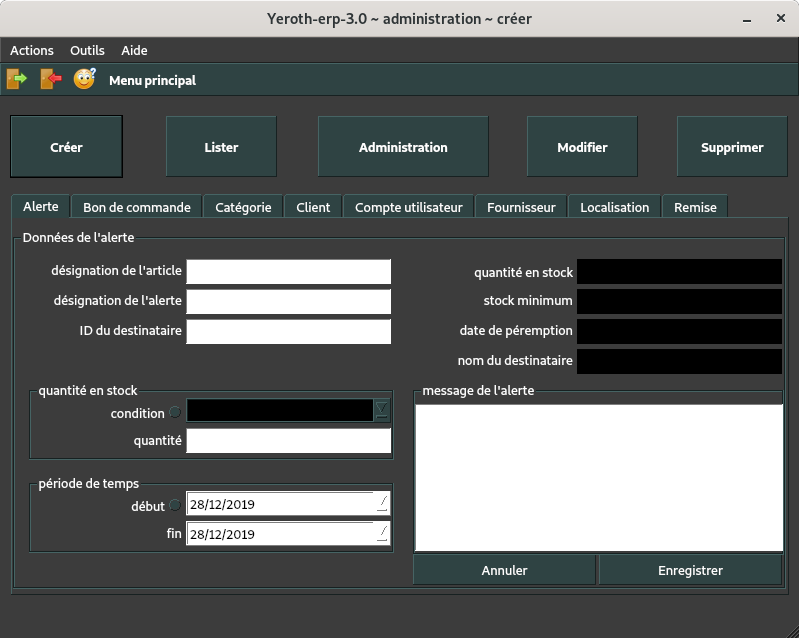
\includegraphics[scale=0.63]{images/yeren-fenetre-creer-alerte.png}
	\caption{La fen\^etre principale pour la cr\'eation d'une alerte.}
	\label{fig:yeren-fenetre-creer-alerte}
\end{figure}

le syst\`eme d'alertes sur les stocks permet aux
utilisateurs de contr\^oler \emph{les dates de
p\'eremption des stocks},
ainsi que \emph{les quantit\'es d'articles en stock}.

\yeren d\'efinit deux types d'alertes sur les stocks:
\begin{enumerate}[1)]
	\item \textbf{les alertes sur une quantit\'e en stock}
	\item \textbf{les alertes sur une p\'eriode de temps}.\\
\end{enumerate}

L'interface de \yeren pour cr\'eer des alertes a deux
\emph{boutons de radio}~\footnote{les boutons de radio
	permettent de faire des choix exclusifs}:

\begin{enumerate}[1)]
	\item le bouton de radio 'quantit\'e en stock'
	\item le bouton de radio 'p\'eriode de temps'.
\end{enumerate}

%-----------------------------------------------------------

\newpage
\nxsection{Cr\'eer une alerte sur une quantit\'e en stock}\label{sec:alerte-quantite-stock}
\index{cr\'eer une alerte sur une quantit\'e en stock}

\begin{enumerate}[1)]
	\item \`A partir de l'interface graphique de l'acceuil de
		l'administration (voir figure~\ref{fig:fenetre-administrateur}),
		on clique sur l'onglet intitul\'e \textbf{op\'erations}. 
		
	\item Choisir '\textbf{cr\'eer}' dans le '\emph{combo box
		op\'erations}'.
		
	\item Choisir '\textbf{une alerte}' dans le '\emph{combo box
		sujets}'. Vous \^etes automatiquement conduit \`a la fen\^etre
		illustr\'ee sur la figure~\ref{fig:yeren-fenetre-creer-alerte}.	
		
	\item Il est pr\'ef\'erable pour de d'abord	choisir le stock
		pour lequel une alerte doit \^etre cr\'eer.	Pour cela il
		faut choisir sa d\'esignation dans le champs de texte
		'\textbf{d\'esignation de l'article}', qui poss\`ede un
		menu auto-d\'eroulant.\\

		Les informations des champs de textes situ\'ees \`a
		droite du champs de texte '\textbf{d\'esignation de l'article}'
		sont non modifiables et affichent des valeurs en fonction
		du stock de l'article s\'electionn\'e:
		\begin{enumerate} [1)]
			\item quantit\'e en stock
			\item quantit\'e minimale (stock)
			\item date de p\'eremption.		
		\end{enumerate}

		Ces informations aident \`a param\'etrer l'alerte.

	\item Donner une d\'esignation \`a l'alerte	en remplissant
		le champs de texte '\textbf{d\'esignation de l'alerte}'.
		
	\item Choisir un destinataire qui recevra le message de
		l'alerte lorsque celle-ci sera d\'eclench\'ee.
		Ceci se fait dans le champs de texte '\textbf{ID du destinataire}',
		qui poss\`ede un menu auto-d\'eroulant.\\
		
		Le nom complet du destinataire est affich\'e automatiquement
		dans le champs de texte '\textbf{nom du destinataire}',
		qui est situ\'e juste \`a droite du champs de texte
		'\textbf{ID du destinataire}'.
		
	\item Choisir le type d'alerte:	\emphbf{quantit\'e en stock}
		en cliquant sur la bouton radio '\textbf{condition}' et 
		en \emph{saisissant un nombre dans le champs de texte
		'\textbf{quantit\'e}'}.
		
	\item Remplir le champs de texte '\textbf{Message de l'alerte}'.
		C'est ce message qui sera envoy\'e au destinataire de
		l'alerte lorsque celle-ci sera d\'eclench\'ee.	
		
	\item Achever la proc\'edure en cliquant sur le bouton \bouton{Valider}.
\end{enumerate}

%-----------------------------------------------------------

\newpage
\nxsection{Cr\'eer une alerte sur une p\'eriode de temps}\label{sec:alerte-periode-temps}
\index{cr\'eer une alerte sur une p\'eriode de temps}

\begin{enumerate}[1)]
	\item \`A partir de l'interface graphique de l'acceuil de
		l'administration (voir figure~\ref{fig:fenetre-administrateur}),
		on clique sur l'onglet intitul\'e \textbf{op\'erations}. 
		
	\item Choisir '\textbf{cr\'eer}' dans le '\emph{combo box
		op\'erations}'.
		
	\item Choisir '\textbf{une alerte}' dans le '\emph{combo box
		sujets}'. Vous \^etes automatiquement conduit \`a la fen\^etre
		illustr\'ee sur la figure~\ref{fig:yeren-fenetre-creer-alerte}.	
		
	\item Il est pr\'ef\'erable pour de d'abord	choisir le stock
		pour lequel une alerte doit \^etre cr\'eer.	Pour cela il
		faut choisir sa d\'esignation dans le champs de texte
		'\textbf{d\'esignation de l'article}', qui poss\`ede un
		menu auto-d\'eroulant.\\

		Les informations des champs de textes situ\'ees \`a
		droite du champs de texte '\textbf{d\'esignation de l'article}'
		sont non modifiables et affichent des valeurs en fonction
		du stock de l'article s\'electionn\'e:
		\begin{enumerate} [1)]
			\item quantit\'e en stock
			\item quantit\'e minimale (stock)
			\item date de p\'eremption.		
		\end{enumerate}

		Ces informations aident \`a param\'etrer l'alerte.

	\item Donner une d\'esignation \`a l'alerte	en remplissant
		le champs de texte '\textbf{d\'esignation de l'alerte}'.
		
	\item Choisir un destinataire qui recevra le message de
		l'alerte lorsque celle-ci sera d\'eclench\'ee.
		Ceci se fait dans le champs de texte '\textbf{ID du destinataire}',
		qui poss\`ede un menu auto-d\'eroulant.\\
		
		Le nom complet du destinataire est affich\'e automatiquement
		dans le champs de texte '\textbf{nom du destinataire}',
		qui est situ\'e juste \`a droite du champs de texte
		'\textbf{ID du destinataire}'.
		
	\item Choisir le type d'alerte:	\emphbf{p\'eriode de temps}
		en cliquant sur la bouton radio '\textbf{d\'ebut}' et 
		en choisissant \emph{les dates de d\'ebut et de fin de
		la p\'eriode de temps pendant laquelle l'alerte sera active}.
		
	\item Remplir le champs de texte '\textbf{Message de l'alerte}'.
		C'est ce message qui sera envoy\'e au destinataire de
		l'alerte lorsque celle-ci sera d\'eclench\'ee.	
		
	\item Achever la proc\'edure en cliquant sur le bouton \bouton{Valider}.
\end{enumerate}

%-----------------------------------------------------------

\newpage
\nxsection{Voir toutes les alertes qu'un utilisateur
 a re\c{c}u~\textcolor{blue}{*}}\label{sec:voire-toutes-alertes}
\index{voir toutes les alertes qu'un utilisateur a re\c{c}u }

\textcolor{blue}{*: Cette fonctionalit\'e est exclusivement
	r\'eserv\'ee aux utilisateurs \manager.}

Pour voire toutes les alertes qui lui sont destin\'ees, l'utilisateur
doit accomplir les actions suivantes \`a partir de toutes fen\^etre
ayant le lien '\textbf{Alertes}' dans sa barre de menu:
\begin{enumerate}[1)]
	\item cliquer sur le lien '\textbf{Alertes}' qui est situ\'e
	dans la barre de menu. Ce lien se retrouve dans toutes les
	fen\^etres concernant la gestion des stocks
	
	\item un utilisateur a aussi acc\`es aux alertes qui lui sont destin\'ees en cliquant sur le lien '\textbf{Alertes}' que
	l'on retrouve dans le menu d\'eroulant \textbf{Outils}.
\end{enumerate}

%-----------------------------------------------------------

\nxsection{Voir les d\'etails d'une alerte}\label{sec:voire-details-alerte}
\index{voir les d\'etails d'une alerte}

L'utilisateur doit accomplir les actions suivantes \`a
partir de toutes fen\^etre ayant le lien '\textbf{Alertes}'
dans sa barre de menu:

\begin{enumerate}[1)]
	\item cliquer sur le lien '\textbf{Alertes}' qui est situ\'e
	dans la barre de menu. Ce lien se retrouve dans toutes les
	fen\^etres concernant la gestion des stocks
		
	\item ensuite, s\'electioner dans l'onglet '\textbf{Alertes}'
		l'alerte dont vous souhaiter voire les d\'etails

	\item enfin, cliquer 2 fois cons\'ecutives sur cette alerte.	
\end{enumerate}

%-----------------------------------------------------------

\nxsection{Marquer une alerte comme r\'esolue~\textcolor{blue}{*}}
\index{marquer une alerte comme r\'esolue}

\textcolor{blue}{*: Cette fonctionalit\'e est exclusivement
	r\'eserv\'ee aux utilisateurs \manager.}

L'utilisateur doit accomplir les actions suivantes \`a
partir de toutes fen\^etre ayant le lien '\textbf{Alertes}'
dans sa barre de menu:

\begin{enumerate}[1)]
	\item cliquer sur le lien '\textbf{Alertes}' qui est situ\'e
	dans la barre de menu. Ce lien se retrouve dans toutes les
	fen\^etres concernant la gestion des stocks
		
	\item ensuite, s\'electioner dans l'onglet '\textbf{Alertes}'
		l'alerte dont vous souhaiter voire les d\'etails

	\item enfin, cliquez sur le bouton \bouton{Marquer r\'esolue}.	
\end{enumerate}

%-----------------------------------------------------------
\newpage
\nxsection{Supprimer une alerte~\textcolor{blue}{*}}
\index{supprimer une alerte}

\textcolor{blue}{*: Cette fonctionalit\'e est exclusivement
		r\'eserv\'ee aux utilisateurs \manager.}

L'utilisateur doit accomplir les actions suivantes \`a
partir de toutes fen\^etre ayant le lien '\textbf{Alertes}'
dans sa barre de menu:

\begin{enumerate}[1)]
	\item cliquer sur le lien '\textbf{Alertes}' qui est situ\'e
	dans la barre de menu. Ce lien se retrouve dans toutes les
	fen\^etres concernant la gestion des stocks
		
	\item ensuite, s\'electioner dans l'onglet '\textbf{Alertes}'
		l'alerte dont vous souhaiter voire les d\'etails

	\item enfin, cliquez sur le bouton \bouton{Supprimer une alerte}.
\end{enumerate}
